\documentclass[a4paper]{article}

\usepackage[fontset=fandol]{ctex}
\usepackage{amsmath, amssymb}
\usepackage{graphicx}
\usepackage[margin=2.3cm]{geometry}
\usepackage[most]{tcolorbox}
\usepackage{listings}
\usepackage{hyperref}
\usepackage{booktabs}
\usepackage{float}
\usepackage{xcolor}

\lstset{
    language=Python,
    basicstyle=\ttfamily\small,
    keywordstyle=\color{blue},
    stringstyle=\color{red!60!black},
    commentstyle=\color{green!50!black},
    breaklines=true,
    frame=single,
    numbers=left,
    numberstyle=\tiny\color{gray}
}

\newtcolorbox{knowledgebox}[1]{
    enhanced,
    colback=blue!5!white,
    colframe=blue!70!black,
    colbacktitle=blue!70!black,
    coltitle=white,
    fonttitle=\bfseries,
    title=#1,
    sharp corners
}

\newtcolorbox{importantbox}[1]{
    enhanced,
    colback=yellow!10!white,
    colframe=yellow!70!black,
    colbacktitle=yellow!70!black,
    coltitle=black,
    fonttitle=\bfseries,
    title=#1,
    sharp corners
}

\newtcolorbox{warningbox}[1]{
    enhanced,
    colback=red!5!white,
    colframe=red!70!black,
    colbacktitle=red!70!black,
    coltitle=white,
    fonttitle=\bfseries,
    title=#1,
    sharp corners
}

\begin{document}

\begin{titlepage}
\centering
{\Large 课程讲义\par}
\vspace{1.2cm}
{\huge\bfseries AlphaProof: when reinforcement learning meets formal mathematics\par}
\vspace{0.6cm}
{\Large CS294/194-280: Advanced Large Language Model Agents\par}
\vspace{0.4cm}
{\large Thomas Hubert, Google DeepMind\par}
\vspace{0.4cm}
{\large 中文教材化讲义 / Codex Harness Build\par}
\vspace{0.8cm}
\includegraphics[width=0.84\textwidth,height=0.38\textheight,keepaspectratio]{cover.jpg}\par
\vfill
\begin{tcolorbox}[width=0.92\textwidth,colback=black!2!white,colframe=black!60,sharp corners]
\textbf{课程页}：\href{https://rdi.berkeley.edu/adv-llm-agents/sp25}{Berkeley RDI SP25 course page}\par
\textbf{录播}：\href{https://www.youtube.com/live/3gaEMscOMAU}{YouTube recording}\par
\textbf{slides}：\href{https://rdi.berkeley.edu/adv-llm-agents/slides/alphaproof.pdf}{alphaproof.pdf}\par
\textbf{补充 readings}：AlphaZero / The Future of Mathematics?
\end{tcolorbox}
\end{titlepage}

\tableofcontents
\newpage

\section{本讲学习目标}

本讲回答的是一个比“IMO 上拿了多少分”更深的问题：\textbf{为什么形式数学（formal mathematics）可能成为高级 LLM agent 最理想的长期环境之一？} 读完本讲后，读者应当能回答：

\begin{itemize}
\item informal reasoning、formal specification、verification、theorem proving、proof search 之间到底有什么边界。
\item 为什么 Lean 能把数学题变成 agent 可交互的环境，而不只是一个排版不同的证明语言。
\item AlphaZero 的哪些 ingredient 被 AlphaProof 继承，哪些没有。
\item 为什么 perfect verification 很有吸引力，但 formalization bottleneck 仍是决定性瓶颈。
\item test-time RL 在 theorem proving 里是什么意思，它与普通采样或 beam search 有什么区别。
\end{itemize}

\section{背景与问题设置}

\subsection{为什么 advanced agents 课程会讲 formal mathematics}

讲者一开始并没有直接谈模型，而是先谈数学的历史位置。原因是：数学既要求\textbf{推理与规划（reasoning and planning）}，又要求\textbf{抽象与泛化（abstraction and generalisation）}，同时还具备开放世界复杂度。很多 agent benchmark 都是在封闭环境里测“会不会操作”，而数学更像是在测“能不能持续构造和验证新知识”。

\begin{figure}[H]
\centering
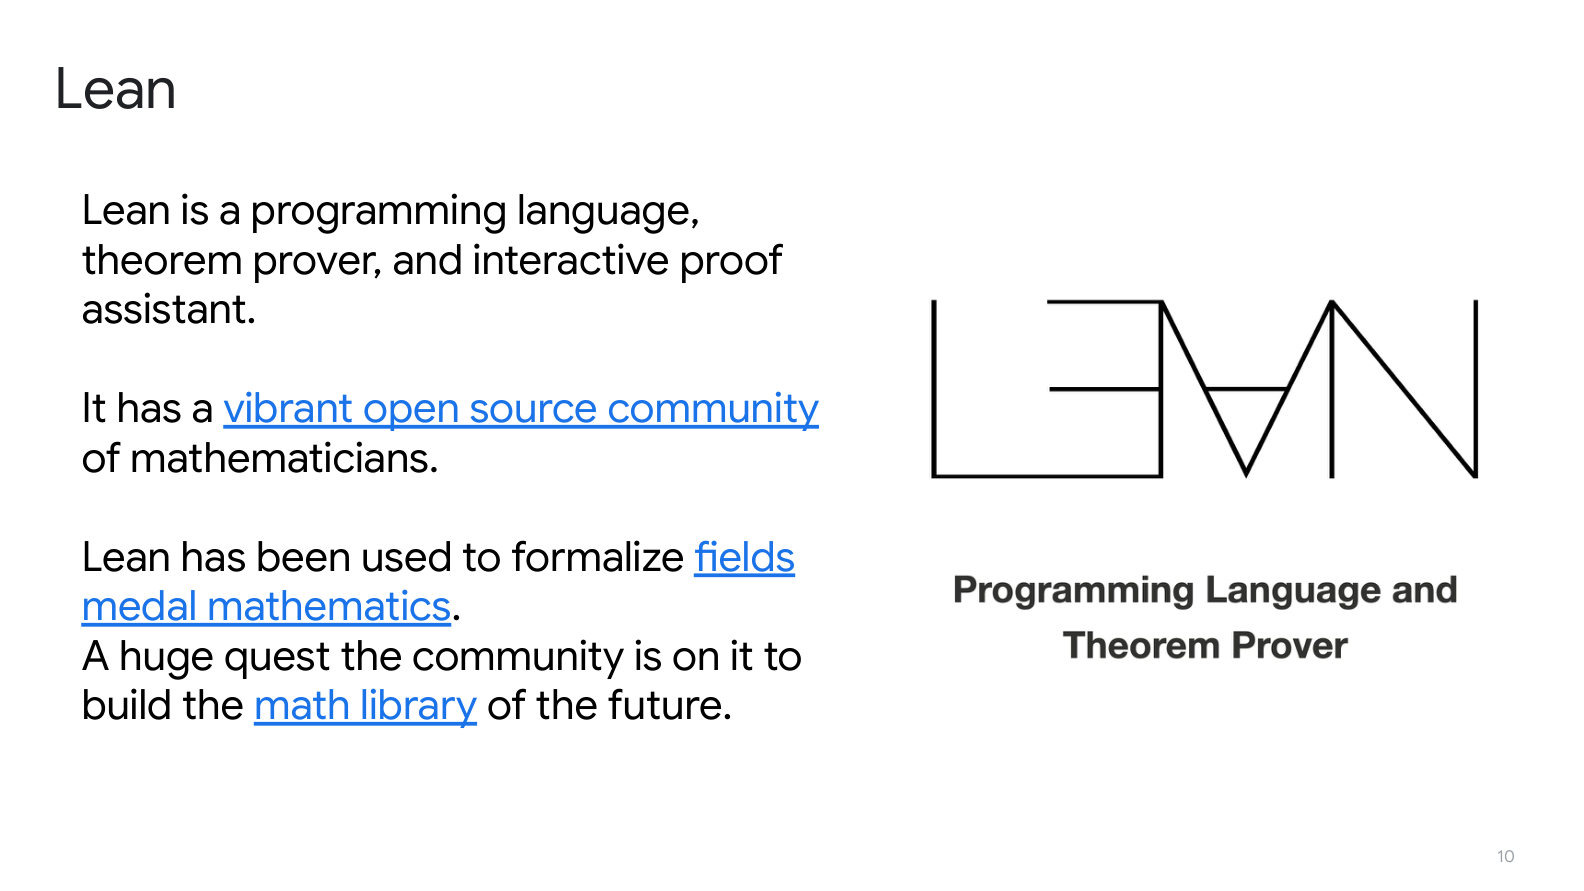
\includegraphics[width=0.82\textwidth]{figures/lec08_fig_001.png}
\caption{Lean 的统一角色：编程语言、定理证明器和交互式 proof assistant。}
\end{figure}

这也是本讲和前几讲的连接点。L01 讨论的是 inference-time computation 如何改善 reasoning；L08 进一步指出：如果没有一个能提供可靠反馈的环境，推理再长也很难被真正检查。形式数学的重要性恰恰在于，它把“我觉得这个证明对”变成“proof checker 能否接受这条状态转移链”。

\subsection{从数学史到形式化：为什么 formal mathematics 不是怪异小众工具}

Slides 用几页历史材料提醒读者：数学本身就是一门不断走向更高\textbf{符号化、形式化、可传递性}的学科。从古希腊对证明的重视，到代数符号逐步取代长篇自然语言，再到现代 proof assistant 的出现，形式化并不是偏离数学，而是把数学中最核心的“可检查性”推到机器层面。

\begin{figure}[H]
\centering
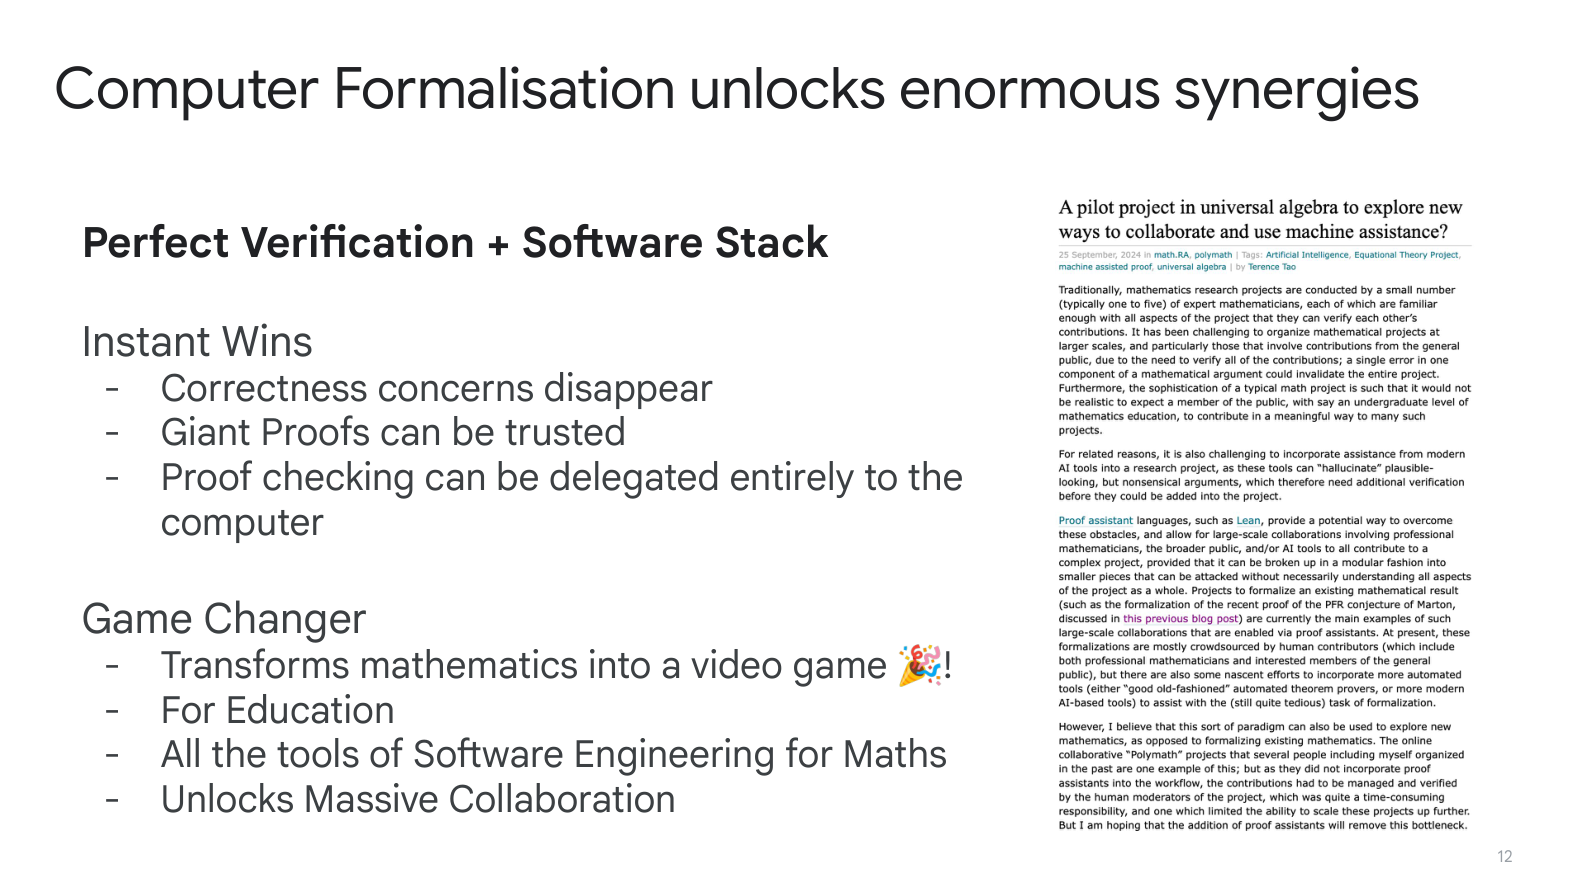
\includegraphics[width=0.80\textwidth]{figures/lec08_fig_002.png}
\caption{形式化带来的协同效应：验证、复用、自动化和软件栈共同作用。}
\end{figure}

讲者把 formalization 的收益总结为几类。第一，\textbf{rigor and clarity}：很多在人类交流中默认跳过的步骤，到了 proof assistant 里必须补齐。第二，\textbf{efficiency and communication}：一旦某个 lemma 进入库，它就不再只是论文中的文字，而是可重用的软件对象。第三，\textbf{unification}：不同领域的证明可以在统一的 formal language 中组合。

\begin{importantbox}{不要把 formalization 理解成“多打一遍字”}
formalization 的价值不在于把自然语言拷贝成另一种语法，而在于把证明过程变成可执行、可组合、可自动检查的计算对象。对 agent 而言，这意味着状态、动作和反馈第一次被严密地固定了下来。
\end{importantbox}

\subsection{但为什么 formal mathematics 直到现在都没有普及}

这也是 lecture 非常诚实的一点：讲者没有把 Lean 说成“已经成熟得足以接管数学研究”。Slides 明确列出 adoption 障碍：学习曲线陡峭，formalization 时间投入巨大，Mathlib 的覆盖并不均匀，很多研究数学对象仍缺乏良好库支持。

\begin{figure}[H]
\centering
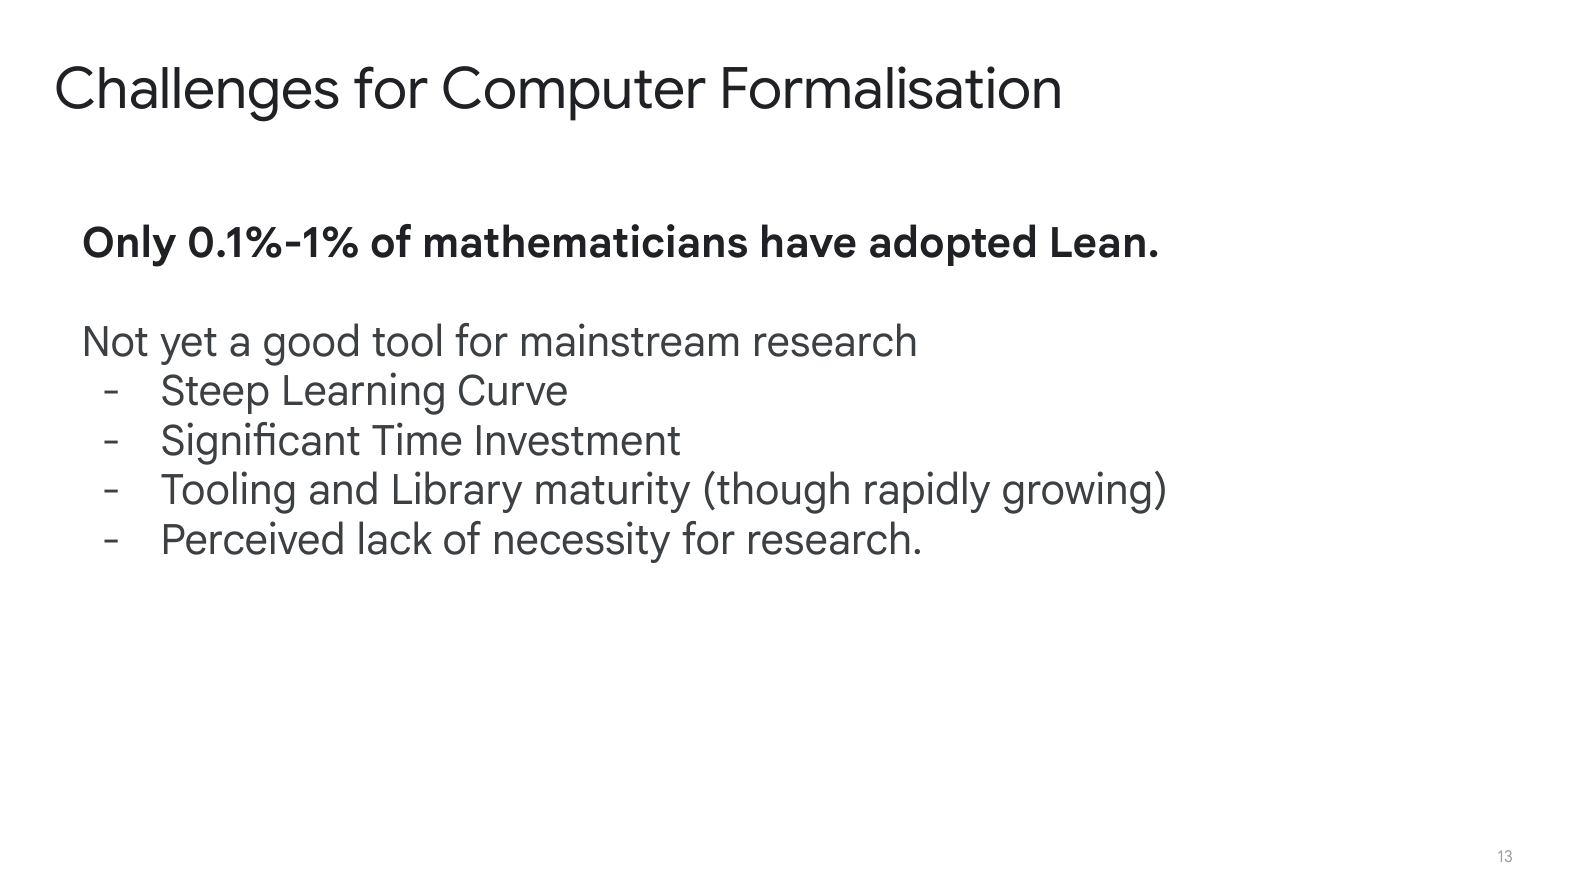
\includegraphics[width=0.82\textwidth]{figures/lec08_fig_003.png}
\caption{Formal mathematics 的现实成本：学习门槛、时间投入与库覆盖。}
\end{figure}

这正是本讲后续所有技术设计的前提。只要 formalization 仍然昂贵，\textbf{“能否求证”}和\textbf{“能否把题目表示出来”}就是两件不同的事。后者是 \textbf{formal specification} 或 \textbf{autoformalization} 问题，前者才是 \textbf{theorem proving} 或 \textbf{proof search} 问题。二者都依赖 verification，但不能混为一谈。

\section{核心概念与术语}

\begin{itemize}
\item \textbf{informal reasoning}：自然语言里的推理草图、启发式解释或数学直觉，通常允许省略步骤。
\item \textbf{formal specification}：把问题陈述翻译成 Lean/Isabelle 中 machine-checkable 的定理陈述。
\item \textbf{verification}：给定 formal statement 和 candidate proof，让 proof checker 判断它是否合法。
\item \textbf{theorem proving}：在 formal system 内搜索一条满足 checker 的证明。
\item \textbf{proof search}：对 proof states、tactics 或 proof tree 进行系统探索的算法过程，可以是 sampling、beam search、MCTS 或 RL-guided search。
\item \textbf{autoformalization}：把自然语言数学自动翻译成 formal theorem 或 formal proof；这是 theorem proving 的前置步骤之一，但不是同一个问题。
\end{itemize}

\begin{knowledgebox}{本讲最关键的区分}
verification 负责“验”；theorem proving 负责“找”；autoformalization 负责“写成可验的形式”。一个系统即便 verification 完美，如果 formalization 很差，也仍然无法把真实数学问题稳定送进 proving 环节。
\end{knowledgebox}

\section{主体讲解：为什么 AlphaZero 可以迁移到数学}

\subsection{先把数学看成一个环境，而不是一堆题目}

Slides 在中段先回顾强化学习的标准四元组：状态、动作、观察、奖励。这个回顾的目的，是为了把 proof assistant 重新解释为一个\textbf{可交互环境}。在 Lean 里，当前 proof goal、上下文假设和局部变量共同组成状态；应用某个 tactic 就是动作；proof state 是否前进、是否报错，就是环境反馈。

\begin{figure}[H]
\centering
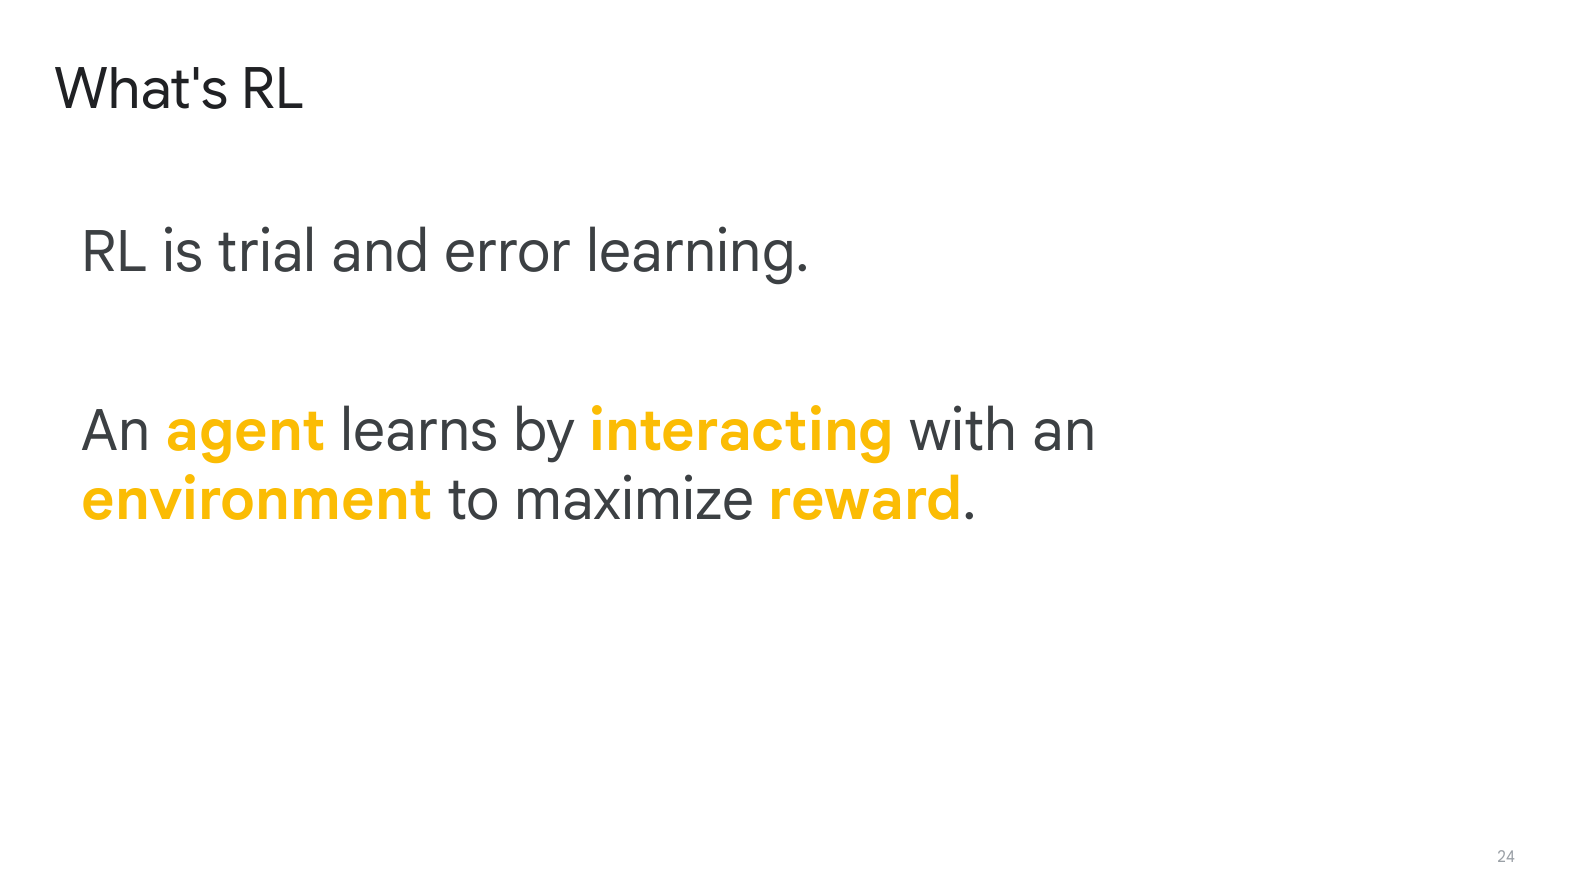
\includegraphics[width=0.76\textwidth]{figures/lec08_fig_004.png}
\caption{把 proof assistant 重述成 RL 环境。}
\end{figure}

如果把 prover 策略记为 $\pi$，那么最粗粒度的目标可写成
\[
\pi^{\star} = \arg\max_{\pi} \mathbb{E}_{\tau \sim \pi}\left[\sum_{t=0}^{T} r_t\right].
\]
这里 $\tau$ 是一条 proof-search 轨迹，$r_t$ 来自 Lean checker 或相关辅助模块给出的 grounded signal。这个式子当然没有捕捉 theorem proving 的全部结构，但它把核心直觉说清楚了：\textbf{proof search 不是散文创作，而是带有可检查状态转移的 sequential decision-making。}

\subsection{AlphaZero recipe 的四个 ingredient}

讲者随后回顾 Alpha 系列系统的共同 recipe：\textbf{scaled up trial and error、grounded feedback、search、curriculum}。把这四项映射到数学上，会得到非常具体的工程判断。

\begin{figure}[H]
\centering
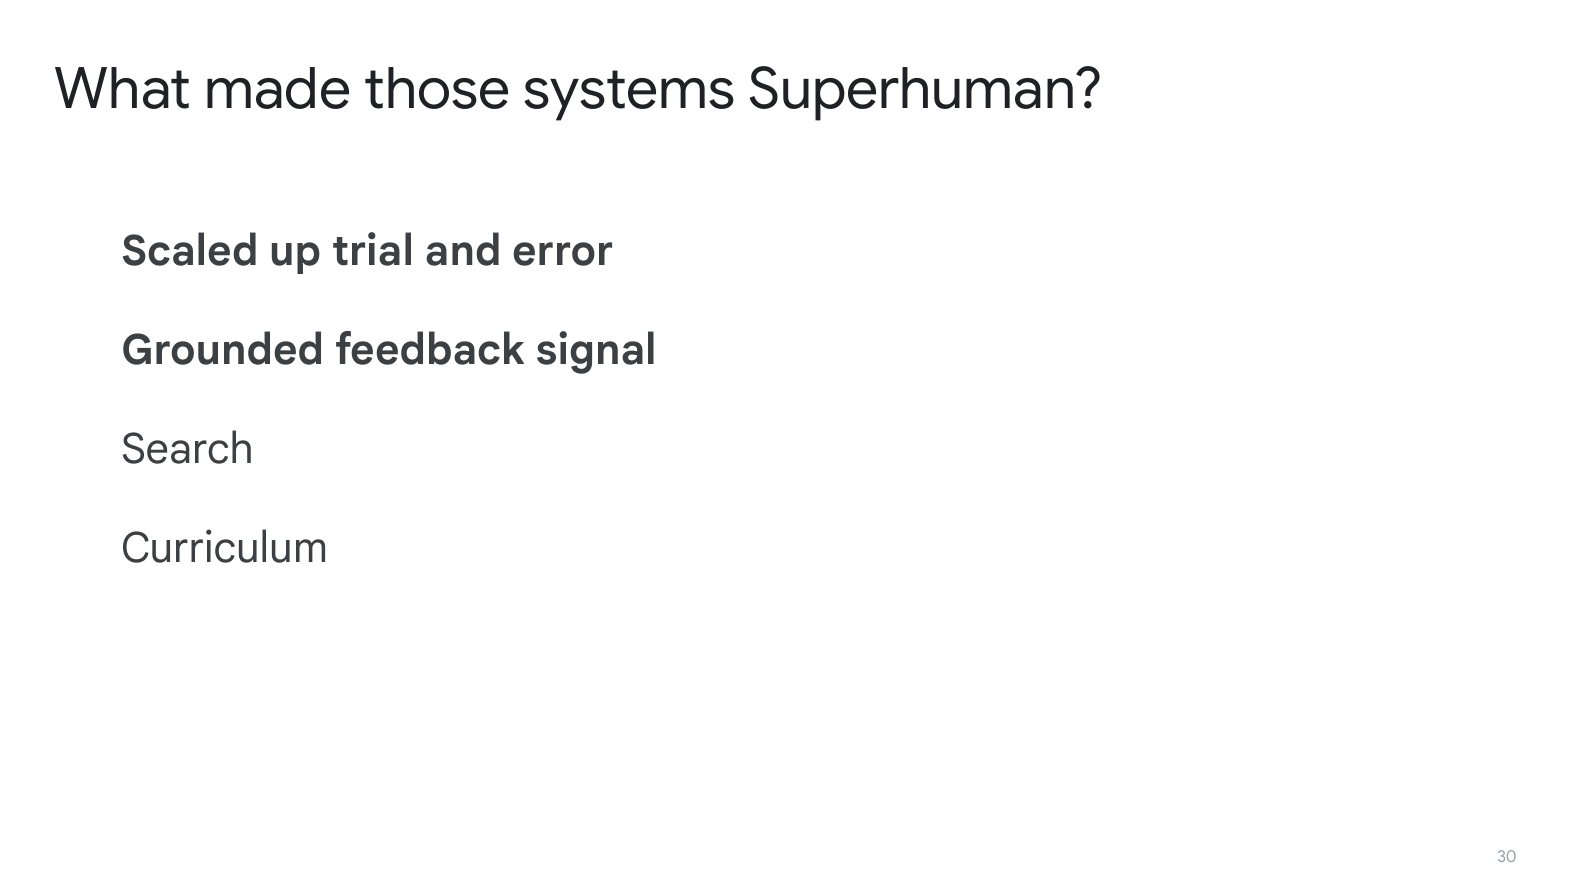
\includegraphics[width=0.82\textwidth]{figures/lec08_fig_005.png}
\caption{Alpha 系列 recipe 的四个 ingredient。}
\end{figure}

\begin{itemize}
\item \textbf{trial and error}：不断尝试 tactics、构造 proof branches、回溯失败路径。
\item \textbf{grounded feedback}：Lean checker 对每一步 state transition 给出精确反馈，不靠人工偏好打分。
\item \textbf{search}：不能只依赖单步 greedy tactic generation，而要在 proof tree 上做更全局的探索。
\item \textbf{curriculum}：先在已有 formal corpus 与较容易问题上学会 action prior，再逐步进到更难定理。
\end{itemize}

\begin{figure}[H]
\centering
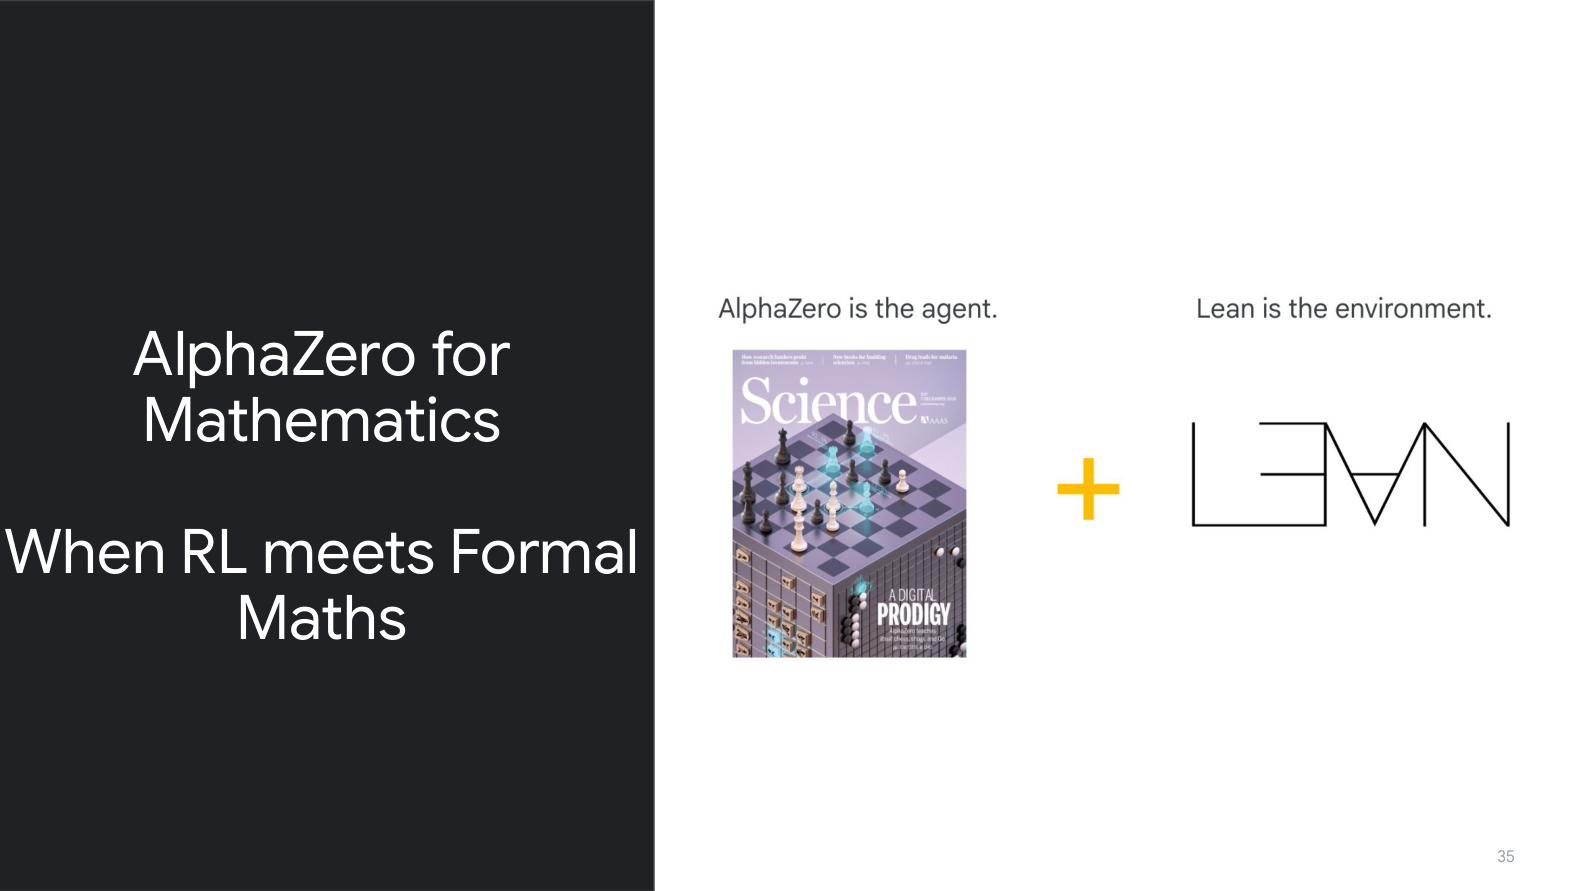
\includegraphics[width=0.80\textwidth]{figures/lec08_fig_006.png}
\caption{“AlphaZero for Mathematics” 是本讲的中心命题。}
\end{figure}

如果采用 AlphaZero 风格的先验引导搜索，动作选择可抽象成
\[
a^{\star}=\arg\max_{a}\left(Q(s,a)+c\,P_{\theta}(a\mid s)\frac{\sqrt{N(s)}}{1+N(s,a)}\right).
\]
这里 $s$ 是当前 Lean proof state，$a$ 是候选 tactic，$Q(s,a)$ 是 value estimate，$P_{\theta}(a\mid s)$ 是 prover 模型提供的动作先验。直觉上，搜索既不能完全听模型先验，也不能盲目穷举；它要在\textbf{高价值路径利用}与\textbf{低访问路径探索}之间平衡。

\begin{lstlisting}
while budget remains:
    sample candidate tactics from the prover prior P(a|s)
    expand/search promising states with value-guided tree search
    apply a tactic inside Lean
    observe the next proof state and checker feedback
    backpropagate success/failure signals
\end{lstlisting}

\paragraph{为什么朴素 prompting 不够}
若只让模型“直接写完整证明”，它其实是在巨大 action space 中一次性押注整条轨迹。任何一步不合法都会让整条轨迹失效。Proof search 的必要性在于：\textbf{数学证明的中间状态非常重要，且可以被环境检查。}

\subsection{AlphaProof 的 foundational bet：少数据但可验证，值得吗}

这是本讲最有洞见的判断。Slides 明确写出：informal mathematics 拥有大量数据，但不可验证；formal mathematics 拥有较少数据，但可验证。

\begin{figure}[H]
\centering
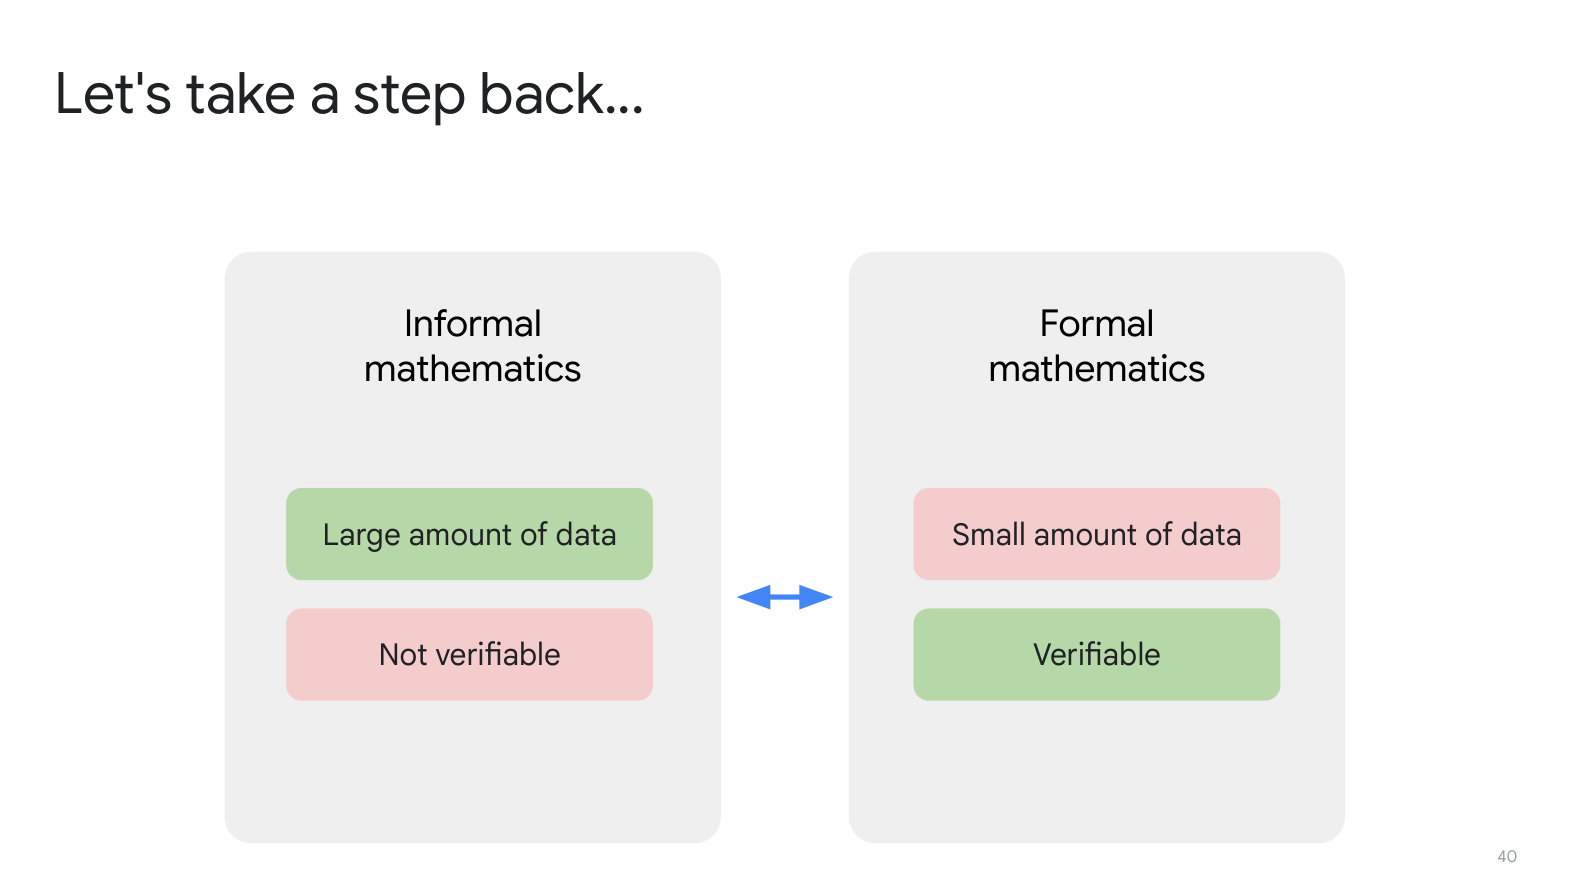
\includegraphics[width=0.78\textwidth]{figures/lec08_fig_007.png}
\caption{数据量与可验证性的张力。}
\end{figure}

\begin{figure}[H]
\centering
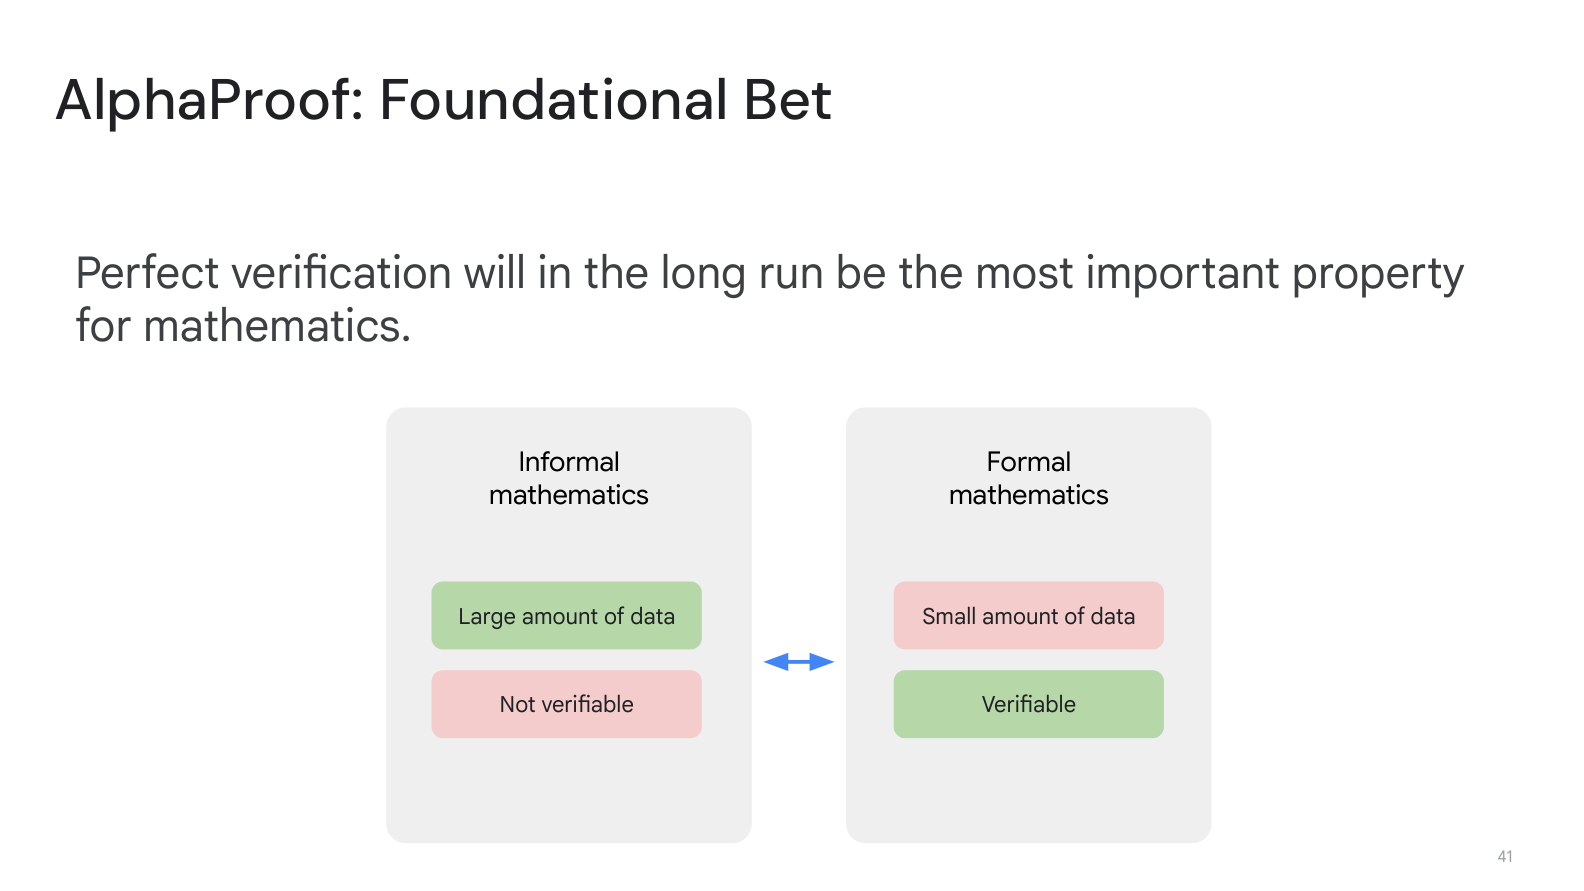
\includegraphics[width=0.78\textwidth]{figures/lec08_fig_008.png}
\caption{“Perfect verification” 是讲者的 foundational bet。}
\end{figure}

这意味着 AlphaProof 的路线不是去追逐最大数据规模，而是在\textbf{验证信号质量}上押注。理由是：长期看，只要 verifier 足够可靠，trial-and-error search 就能被持续扩展；而如果反馈本身不可信，再长的 CoT 和再多的 sampled proofs 也只是不可检验文本。这个判断和前几讲中的一个 recurring theme 是一致的：\textbf{高质量外部反馈比纯自说自话更关键。}

\section{IMO 2024：为什么这是 benchmark，也是系统工程实战}

\subsection{Apollo-style milestone，而不是“数学 AGI 已成”}

讲者把 IMO 2024 比作 Apollo program，并不是说解出 IMO 就等于通用数学家诞生，而是说：在算力、时间和软件栈都受限的现实条件下，能否让系统在一个具有全球可比性的 benchmark 上完成高难任务。

\begin{figure}[H]
\centering
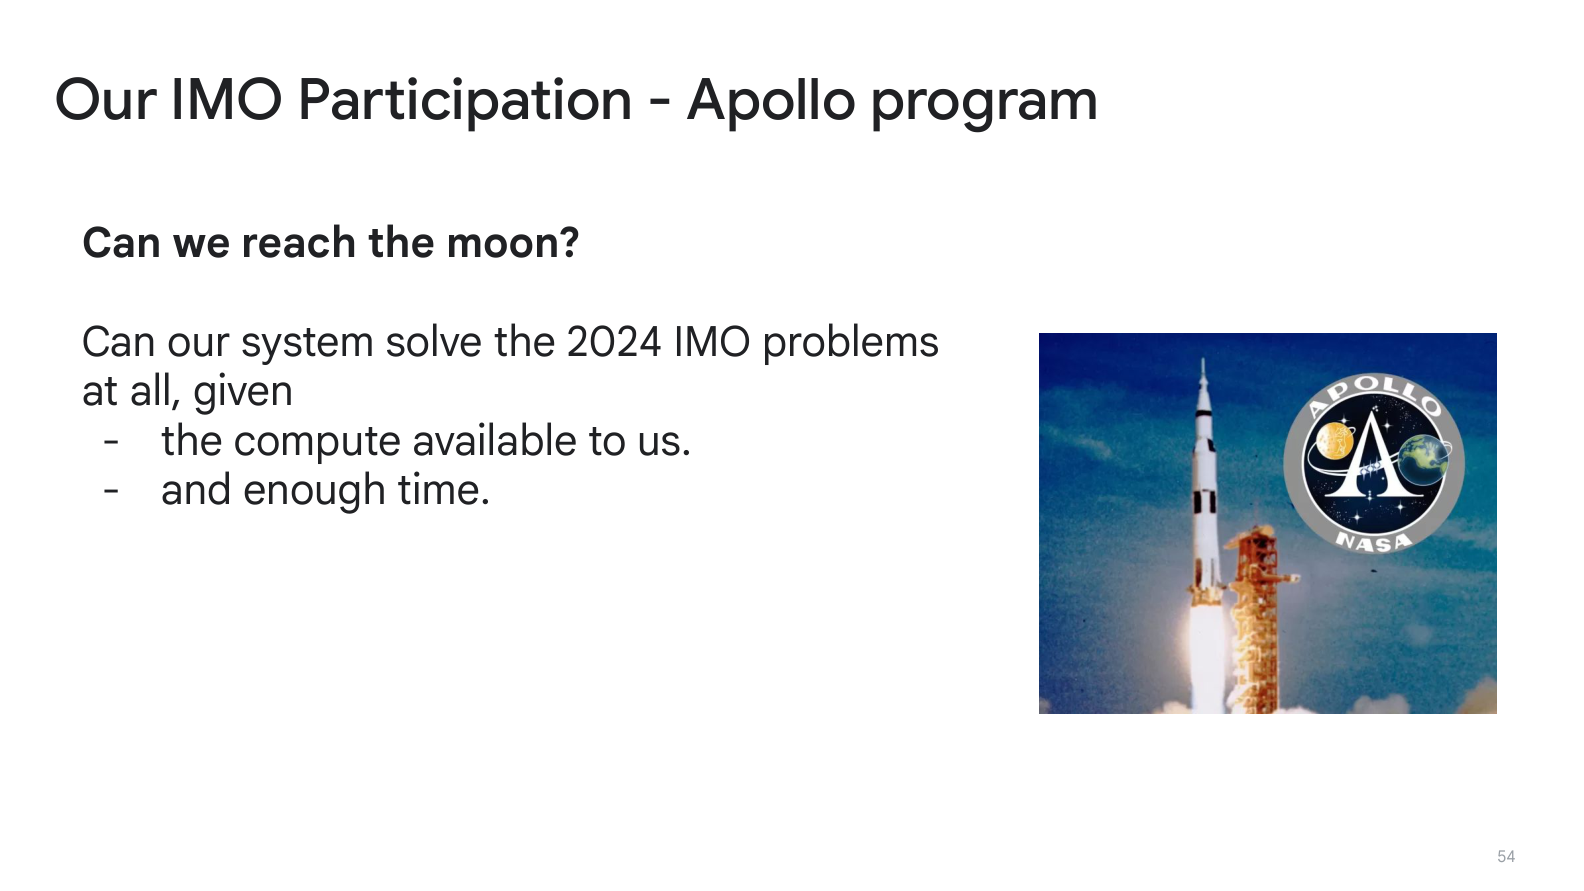
\includegraphics[width=0.82\textwidth]{figures/lec08_fig_009.png}
\caption{IMO 2024 作为 Apollo-style milestone。}
\end{figure}

这一 framing 很重要，因为它重新定义了成功标准。系统不是要证明“数学已经 solved”，而是要证明\textbf{formal verification + search + RL}这条路线具有外部可见的里程碑价值。

\subsection{比赛期间的 protocol：formalization 与 proving 明确分层}

比赛流程页揭示了一个非常重要的工程事实：\textbf{AlphaProof 并不是端到端从自然语言 IMO 题目直接出 formal proof。} 真正的 protocol 包括：专家先将题目 formalize 到 Lean；Gemini 生成大量候选答案；系统用 disprover 去剔除明显错误的猜测；再由 AlphaProof/AlphaGeometry 对剩余候选进行深搜。

\begin{figure}[H]
\centering
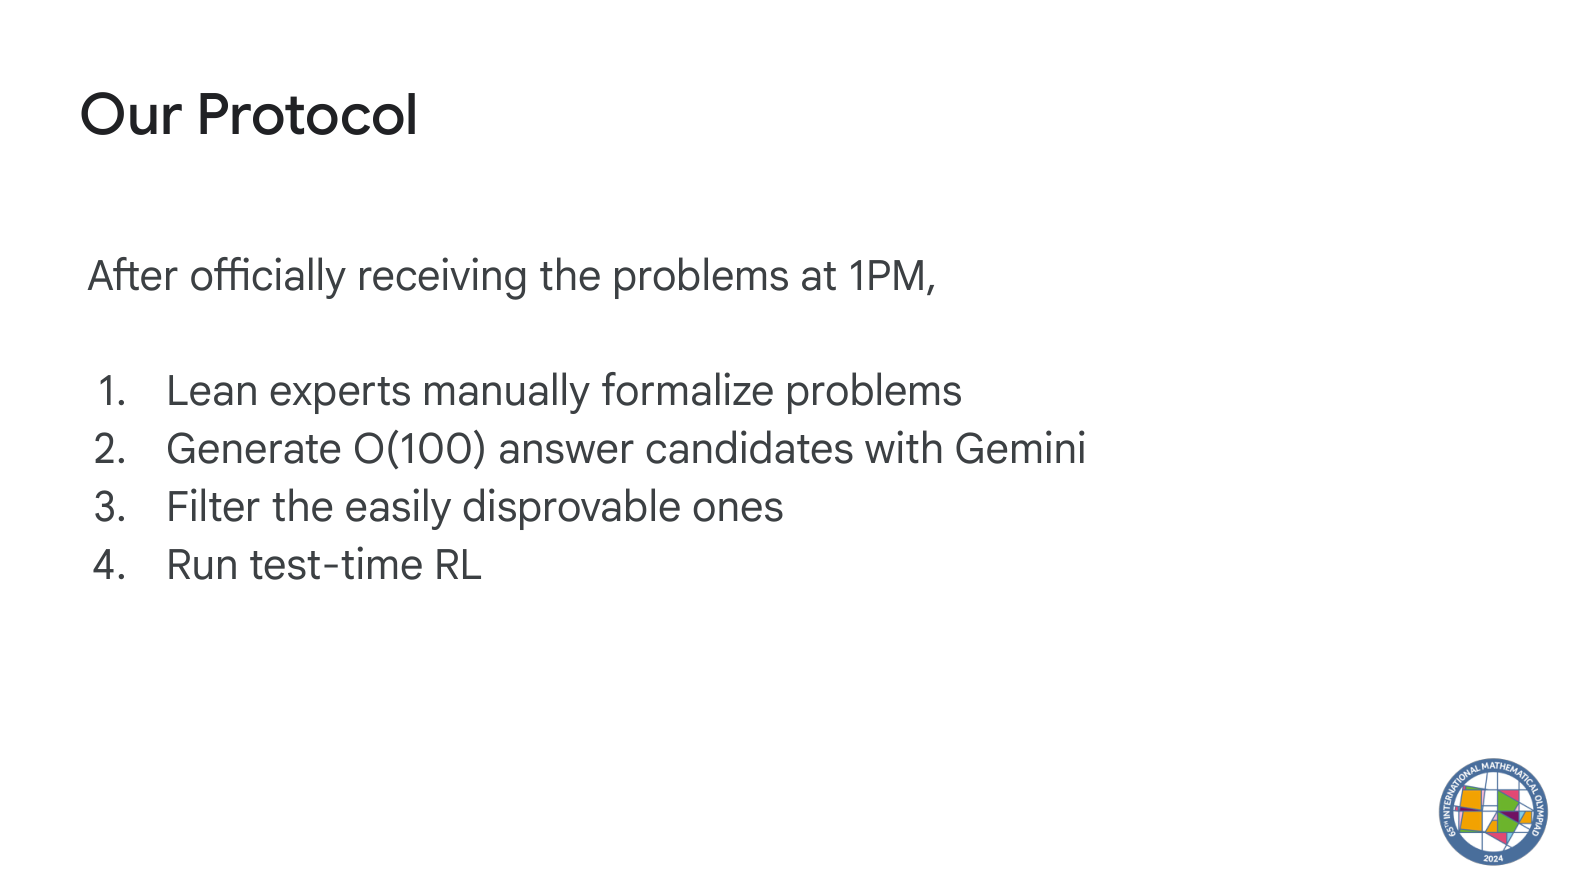
\includegraphics[width=0.86\textwidth]{figures/lec08_fig_010.png}
\caption{比赛日 protocol：manual formalization、candidate generation、disproving 与 proof search 的分工。}
\end{figure}

\begin{lstlisting}
receive official IMO problem
manual Lean formalization by experts
generate O(100) candidate answers with Gemini
use disprover to eliminate easy wrong guesses
run AlphaProof/AlphaGeometry on the remaining candidates and proofs
\end{lstlisting}

这个 protocol 之所以值得细讲，是因为它把\textbf{formal specification} 与 \textbf{theorem proving} 强行拆开。前者仍依赖专家；后者才是 AlphaProof 真正擅长的部分。这既是系统成功的原因，也是当前能力边界最诚实的描述。

\subsection{结果、反例与边界条件}

\begin{figure}[H]
\centering
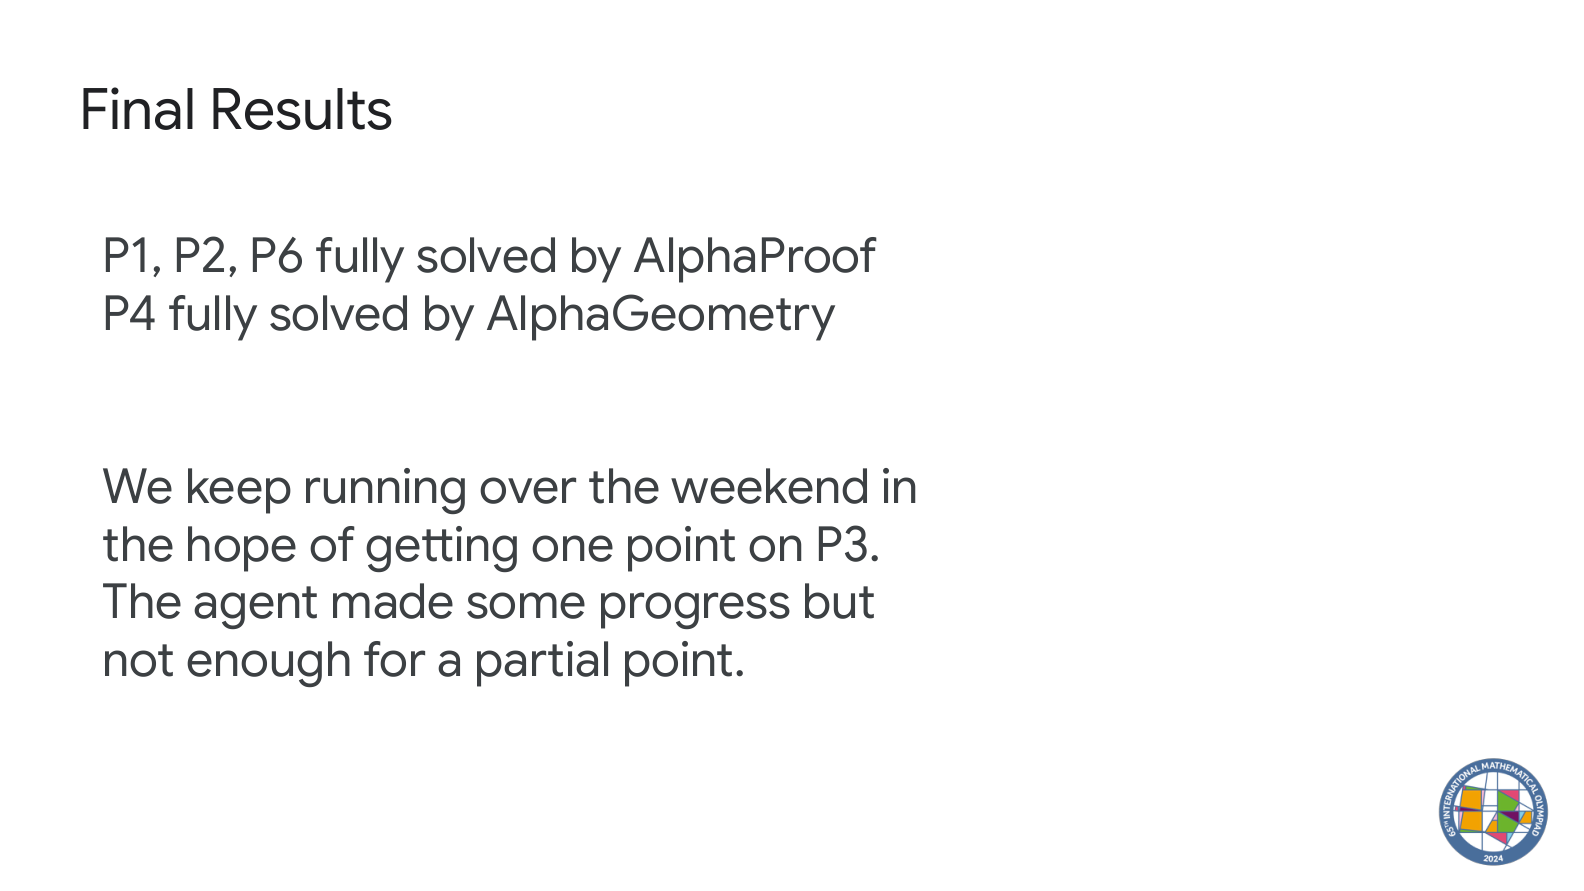
\includegraphics[width=0.84\textwidth]{figures/lec08_fig_011.png}
\caption{AlphaProof 与 AlphaGeometry 在 IMO 2024 的结果。}
\end{figure}

Slides 展示的结果非常强，但更值得注意的是失败分布。P4 几何题需要 AlphaGeometry 才能补上，P3/P5 的组合与几何难点暴露出 Mathlib 覆盖、formalization 难度和 proof-search branching factor 的多重瓶颈。也就是说，\textbf{验证信号完美}并没有自动消除\textbf{表示、建模和搜索}的困难。

\begin{warningbox}{不要把银牌结果误读为“形式数学已被攻克”}
AlphaProof 证明的是：在有 formal environment、强搜索和足够工程投入时，系统能在高难 benchmark 上取得可信成绩。它没有证明：自然语言数学题可以被无缝 formalize，或者开放研究数学已经接近 solved。
\end{warningbox}

\section{AlphaProof 的系统分解：formalizer、prover、search 与 test-time RL}

\subsection{formalizer：把自然语言数学送进 Lean}

Slides 在后半段明确给出 formalizer 接口：输入是自然语言问题或定理，输出是 Lean 中的 formal statement。
\[
\hat{T}_{\mathrm{formal}} = f_{\phi}(x_{\mathrm{informal}}).
\]
其中 $x_{\mathrm{informal}}$ 是自然语言题目，$f_{\phi}$ 是 formalizer，$\hat{T}_{\mathrm{formal}}$ 是转写后的 formal theorem statement。

\begin{figure}[H]
\centering
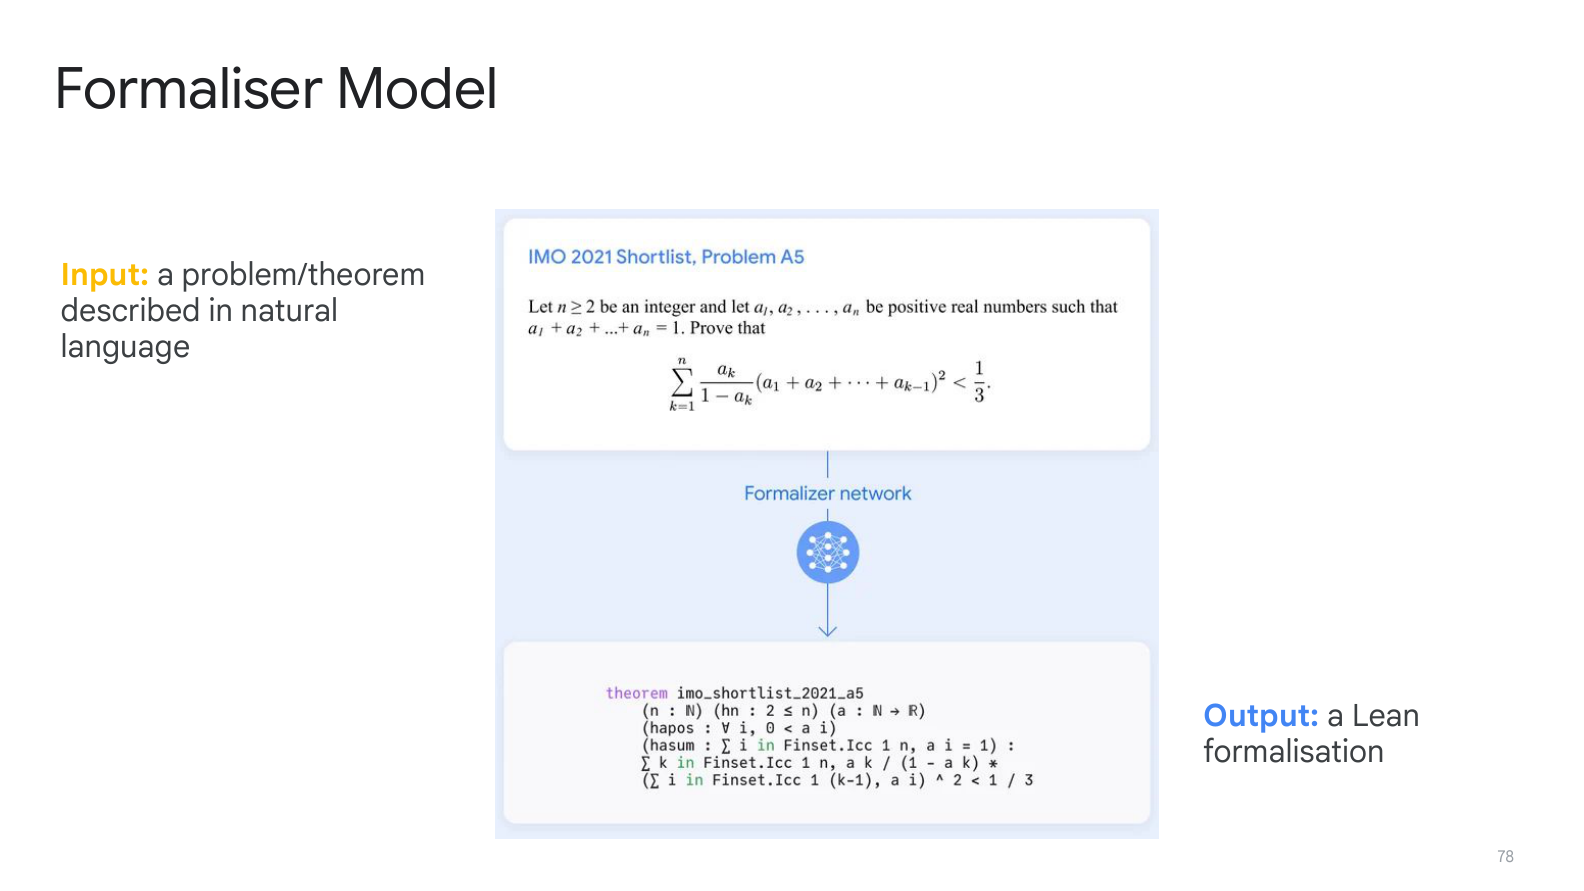
\includegraphics[width=0.78\textwidth]{figures/lec08_fig_012.png}
\caption{Formalizer 的输入输出接口。}
\end{figure}

这一步不等于 proving。它只是在构造“什么才是需要被证明的对象”。为什么这一步困难？因为自然语言问题包含缩写、隐含量词、默认背景知识，有时甚至包含图示或约定俗成的数学写法。形式系统无法容忍这些省略。

\subsection{prover + proof search：在 Lean state/action 空间里行动}

\begin{figure}[H]
\centering
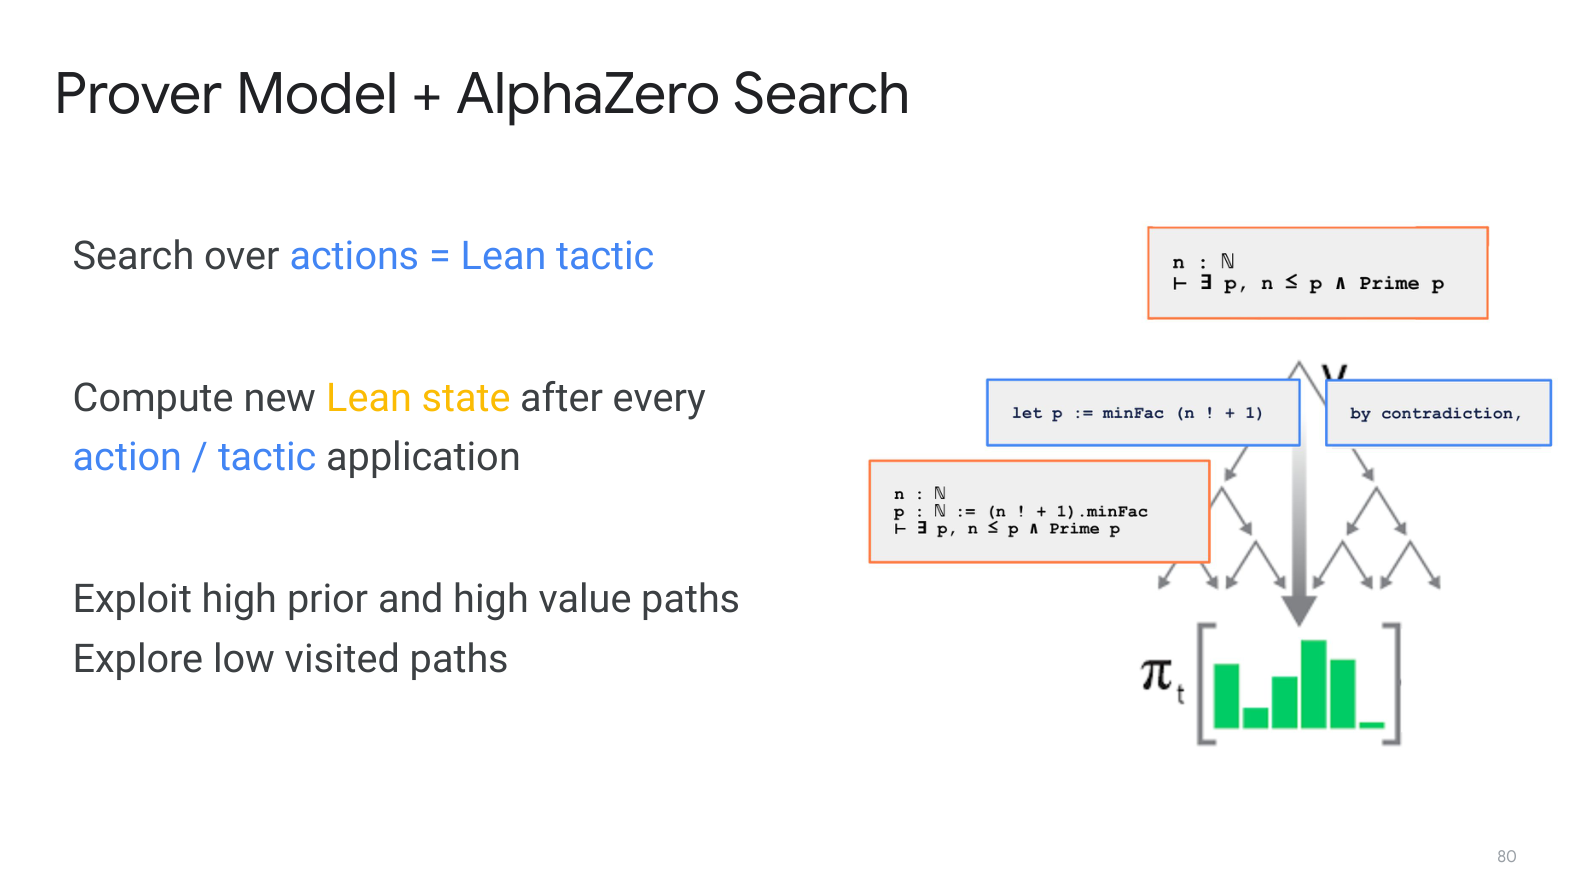
\includegraphics[width=0.82\textwidth]{figures/lec08_fig_013.png}
\caption{Prover 在 Lean 中搜索 tactic。}
\end{figure}

在 theorem proving 阶段，模型不再输出漂亮散文，而是输出 tactics 或证明步骤。每一步都会改变 proof state。这个过程与普通自然语言生成最不同的地方在于：\textbf{每一步都能被环境立即判定是否合法。} 因而 proof search 更接近 game playing 或 program synthesis，而不是开放式写作。

\subsection{AlphaZero-style RL：不只监督模仿，还要从搜索经验里学习}

讲者随后给出训练管线：先用 formalized problems 和 Mathlib 做监督学习，学到 action prior；再在 proof-search 环境中收集 proving/disproving experience，用 RL 继续提升策略。

\begin{figure}[H]
\centering
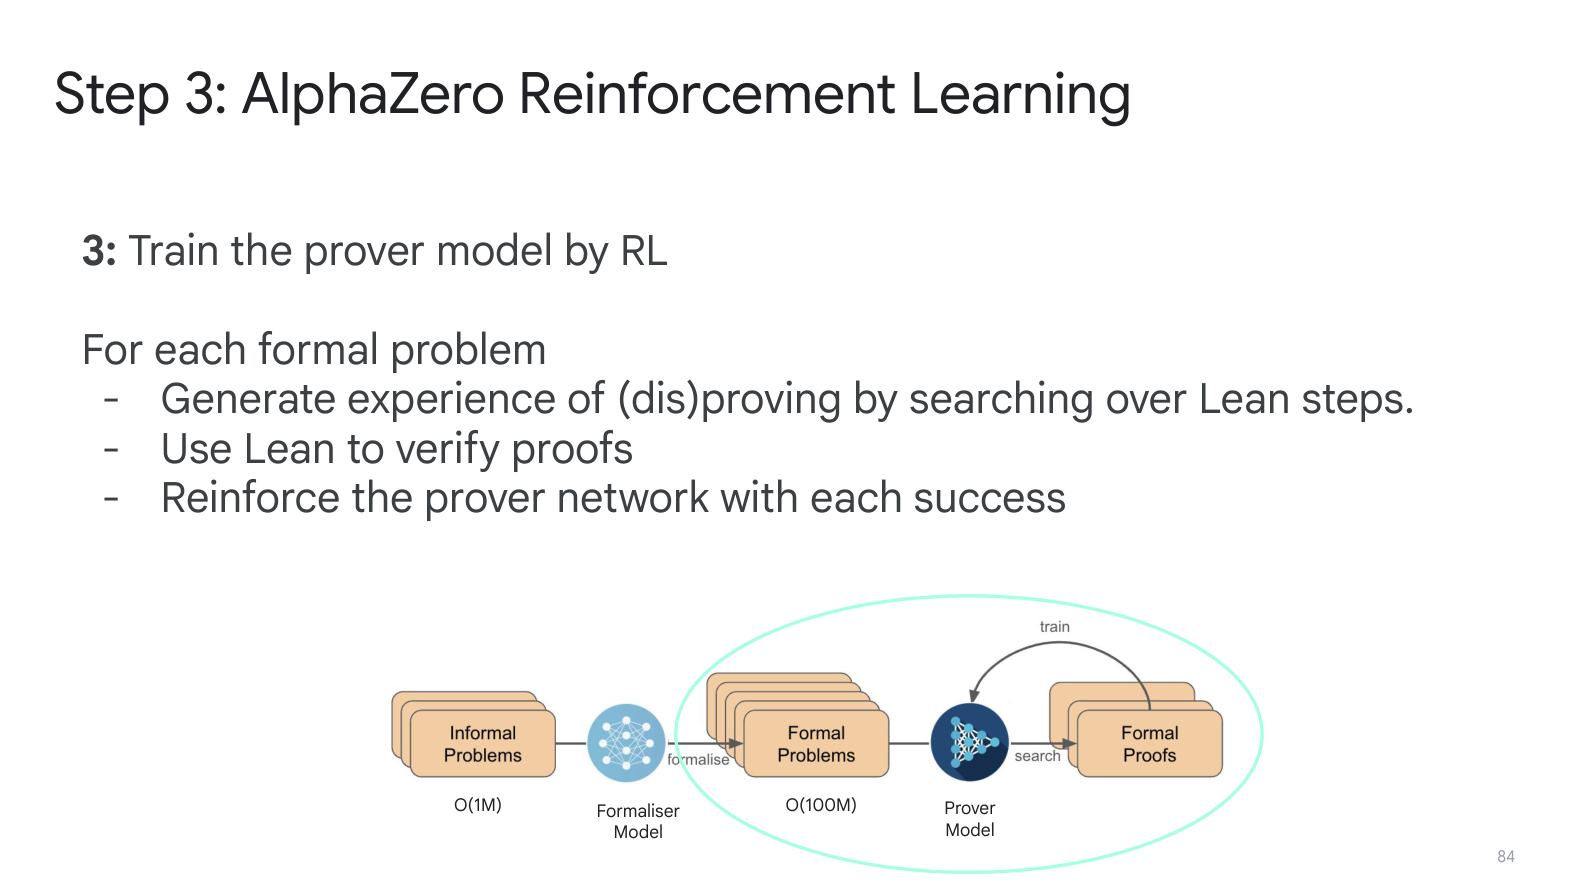
\includegraphics[width=0.84\textwidth]{figures/lec08_fig_014.png}
\caption{AlphaZero-style RL 在 theorem proving 上的经验生成。}
\end{figure}

\begin{lstlisting}
informal problem -> formalizer model -> Lean theorem statement
formal theorem state -> prover model + search -> tactic sequence
Lean checker verifies every state transition and the final proof
\end{lstlisting}

这里的一个重要直觉是：仅做 imitation learning 会把模型限制在现有人类 proofs 分布附近；而 RL 让系统能在 search 中发现\textbf{人类数据里不存在、但被 checker 认可}的新路径。这也是讲者强调“discovering knowledge by themselves”的原因。

\subsection{test-time RL：围绕超难目标问题做局部 specialization}

最有 agent flavor 的部分是 test-time RL。Slides 把它画成一个“problem bubble”：从 generalist checkpoint 出发，在目标难题周围生成变体问题，利用这些局部问题继续 RL，形成更适合该难题附近分布的 specialist。

\begin{figure}[H]
\centering
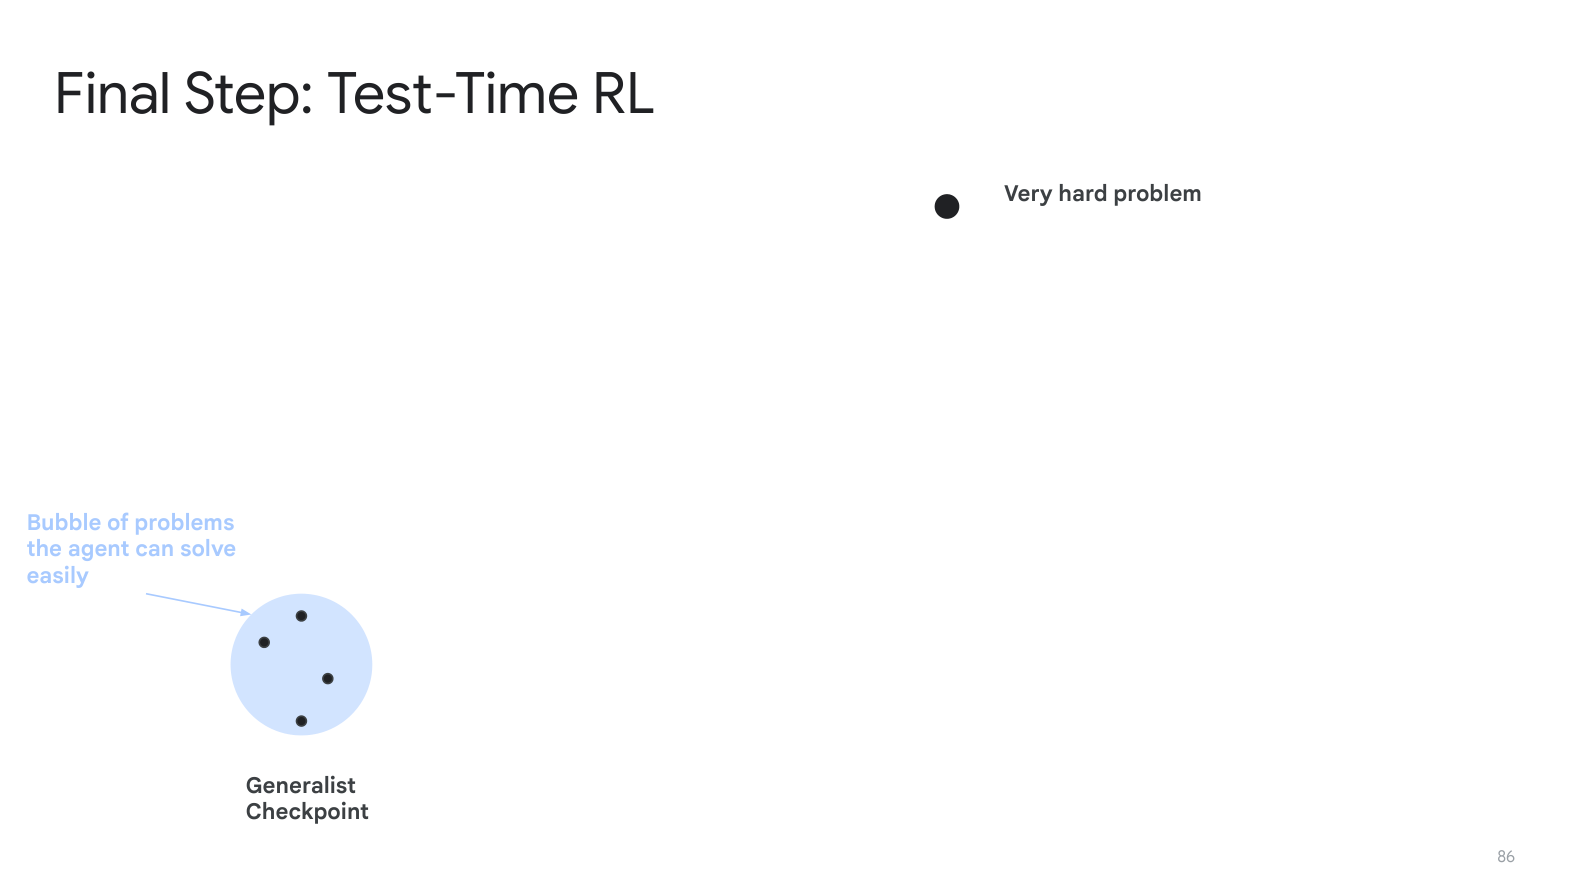
\includegraphics[width=0.82\textwidth]{figures/lec08_fig_015.png}
\caption{从 generalist 到 specialist 的 test-time RL bubble。}
\end{figure}

可抽象为
\[
\theta' = \arg\max_{\theta}\;\mathbb{E}_{\tilde{p}\sim \mathcal{N}(p)}\left[R_{\mathrm{Lean}}\!\left(\pi_{\theta}, \tilde{p}\right)\right].
\]
这里 $p$ 是目标难题，$\mathcal{N}(p)$ 是围绕它构造的变体分布，$R_{\mathrm{Lean}}$ 是 Lean 反馈定义的 reward。直觉是：如果原始问题太难，直接在它上面 RL 信号稀薄；但若能找到与之邻近的一簇可解变体，就能在局部形成有效 curriculum。

\begin{lstlisting}
start from a generalist checkpoint
construct variants around the target hard problem
search and collect proving/disproving experience
update the prover by RL on that local bubble
deploy the specialized checkpoint back onto the target problem
\end{lstlisting}

\paragraph{为什么这不是简单的“多采样一些”}
多采样只是增加宽度，test-time RL 则是在\textbf{改变策略本身}。它让系统在部署时仍保留学习能力，这一点与本课程“agent 不是静态 predictor，而是带有环境反馈闭环的系统”高度一致。

\section{关键论文与课程 readings 的连接}

\subsection{AlphaZero reading：迁移的是 recipe，不是棋盘}

《Mastering Chess and Shogi by Self-Play with a General Reinforcement Learning Algorithm》为本讲提供了最核心的算法祖先。Lecture 真正继承的是一种 harness：强先验模型、search、grounded feedback、自生成经验与 iterative improvement 的闭环。不同之处在于，棋类环境天然可模拟，而数学环境需要 Lean/Mathlib 这样的形式系统来构造。

更具体地说，AlphaZero 给 AlphaProof 提供的不是某个棋类专用 trick，而是三条更一般的系统原则。第一，\textbf{环境必须给出无歧义反馈}，否则 search 与 RL 无法稳定闭环。第二，\textbf{policy/value 与 search 要联动}，单独扩大采样宽度并不等于有效搜索。第三，\textbf{经验生成本身是能力来源}，系统要能从自身 rollouts 中不断积累更有用的 proving data。

但这条迁移也有明确断点。棋类里 legal move checker、终局 reward 和 simulator 都是现成的；形式化数学里，formalization 成本、library coverage 和 tactic/action space 远比棋盘复杂。因此 lecture 把 AlphaZero 当作 ancestor，是为了说明 \emph{recipe continuity}，不是为了暗示 theorem proving 已经像棋类那样“环境完备”。

\subsection{The Future of Mathematics?：生态位与基础设施视角}

这段 reading 不是 benchmark paper，但它解释了为什么 formal mathematics 社区建设本身重要。没有 Lean 教学、Mathlib 沉淀和 formal abstracts 这样的生态基础，AlphaProof 无法把数学变成 machine-actionable environment。换句话说，\textbf{agent 的上限不仅受模型限制，也受环境基础设施成熟度限制。}

这也是本讲和很多“数学 AI demo”最不一样的地方。lecture 并没有把形式化数学当成一个单独 benchmark，而是把它视为一套逐步成熟中的 research infrastructure。Buzzard 那条线强调 curriculum digitization、formal abstracts 和教学生态，其实是在回答一个更底层的问题：\textbf{如果环境本身还没有被系统化整理出来，再强的 proving agent 也只能在很窄的子空间里工作。}

\subsection{把两篇 readings 合在一起看}

把 AlphaZero 和《The Future of Mathematics?》放在一起，能更准确地理解 AlphaProof 的位置。前者解释了为什么 search + policy/value + self-generated data 是强 agent recipe；后者解释了为什么 Lean / Mathlib / formal education community 是使该 recipe 可落地的环境前提。没有前者，AlphaProof 不知道如何在 environment 中学习；没有后者，AlphaProof 连一个可持续扩展的 environment 都没有。

\section{例子、失败模式和边界条件}

\subsection{Formal mathematics 的失败模式}

\begin{itemize}
\item \textbf{representation bottleneck}：题目还没被 formalize，prover 再强也无从行动。
\item \textbf{library bottleneck}：Mathlib 缺什么，系统就很难有效进入对应领域。
\item \textbf{action-space explosion}：tactic 选择空间巨大，局部贪心会迅速陷入死路。
\item \textbf{benchmark overfitting}：若一味围绕某类 Olympiad 题做 specialization，系统可能难以转向开放研究数学。
\end{itemize}

\subsection{与 verification 的关系}

verification 是整个路线成立的底座，但它只回答“这一步是否合法”。它不回答：哪条 proof path 更容易找到？哪个 formalization 最贴近原题？哪种 curriculum 更值得投入算力？因此 verification 是必要条件，不是充分条件。

\section{与前后讲的联系}

与 L01 相比，本讲把“需要外部反馈”这一原则推进到了极致：Lean checker 给出的是几乎无歧义的 grounded feedback。与下一讲 L09 相比，本讲更偏向系统和环境视角；L09 会更细分 autoformalization、theorem proving、retrieval、evaluation gaps 等问题，并系统解释为什么 formal mathematics 不是一个单一任务。

\section{本章小结}

AlphaProof 的重要性，不在于它把一个 benchmark 做到了多高，而在于它展示了 formal mathematics 可以承载高级 agent 的完整闭环：问题表示、状态转移、外部验证、搜索、强化学习和 test-time specialization。它也同样清楚地展示了边界：formalization 成本、Mathlib 覆盖和 proof-search action space 仍然是关键难点。

\section{复习题}

\begin{enumerate}
\item 为什么讲者认为 mathematics 是 intelligence 的 root node？
\item Lean 在 AlphaProof 里分别扮演了哪些角色？
\item AlphaZero recipe 的四个 ingredient 如何映射到 theorem proving？
\item 为什么 perfect verification 依然无法自动解决 formalization bottleneck？
\item test-time RL 与普通多样本采样有什么本质差异？
\end{enumerate}

\section{深入思考题}

\begin{enumerate}
\item 如果未来 autoformalization 大幅进步，AlphaProof 的系统瓶颈会转移到哪里？
\item 在 theorem proving 中，value model、search policy 与 retrieval 分别应承担什么职责？
\item formal mathematics 是否一定比开放世界 web/GUI agent 更适合作为长期 AGI benchmark？为什么？
\end{enumerate}

\section{延伸阅读}

\begin{itemize}
\item \emph{Mastering Chess and Shogi by Self-Play with a General Reinforcement Learning Algorithm}
\item \emph{The Future of Mathematics?}
\item AlphaGeometry / Mathlib / Lean ecosystem materials
\end{itemize}

\end{document}
